\section{Conclusion}

\begin{figure}[t]
\centering
 \subcaptionbox{\label{fig:bit-distrib-rmse-tile}\emph{RMSE}}{{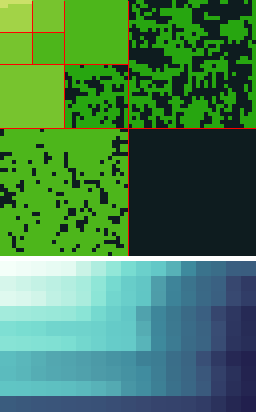
\includegraphics[width=0.32\linewidth]{bit-distrib-rmse-tile}}}
 \subcaptionbox{\label{fig:bit-distrib-laplacian-tile}\emph{Laplacian}}{{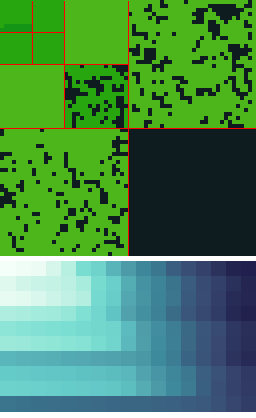
\includegraphics[width=0.32\linewidth]{bit-distrib-laplacian-tile}}}
 \subcaptionbox{\label{fig:bit-distrib-histogram-tile}\emph{histogram}}{ {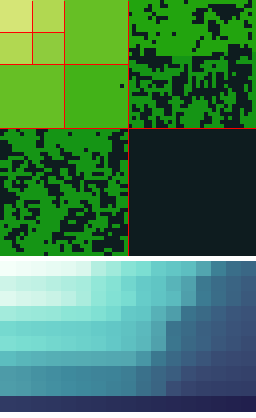
\includegraphics[width=0.32\linewidth]{bit-distrib-histogram-tile}}}
 
\caption{(Top) Bit distribution across subbands at 1.9 bps, and (bottom) corresponding stream
signatures, for the three streams \ssig, \slsg, and \shsg. The data is a 2D slice from
\emph{diffusivity}. The lowest-level subband is in the top-left corner, and subbands are separated
by red lines. The color of each pixel indicates the bit plane at which the corresponding coefficient
is currently at. Bit plane 0 (the most significant) is mapped to the darkest green, and bit plane 16
is mapped to the brightest. It can be observed in both the top and the bottom rows that \shsg
allocates more bits to the lower subbands, while \slsg prefers to stream bits from higher subbands.
\ssig is somewhere in the middle.}
\label{fig:bit-distrib}
\end{figure}

We presented a study of tradeoff between resolution and precision for commonly used derived
scientific quantities such as RMSE, gradient, Laplacian, histogram, and isosurface.
During this study, we covered the gamut of scientific data sets, ranging from simulations
with smooth features or fine scale detail to image data with noisy parts\pavol{do we have plot of image data?}.
We showed that one stream type does not fit all analysis tasks, but some streams perform well
in most of them and may be useful in a new file format design.





We started with an evaluation of contemporary techniques for reducing resolution or precision.
The experiments showed that streaming only in resolution or precision is suboptimal for all
tested queries. We thus developed a tractable greedy algorithm for computing adaptive stream order
based on the particular task. The produced stream significantly\pavol{it would be good to quantify what
significantly means, 2x?} outperforms any stream that has
a fixed streaming order.

After establishing the greedy algorithm for computing a stream, we focused on each query and
investigated which queries have similar streams. This approach is important because if two streams
are very similar, we can precompute the stream order and apply the same ordering to different
queries.

For example, we learned that the RMSE stream is akin to the gradient stream, and thus only one
needs to be computed. Moreover, since RMSE optimizes for the function, the stream alongside
a good gradient approaches the function itself. In contrast, the gradient ignores the constant offest
of all samples, resulting in an inferior RMSE.


These results should be considered when designing a file format for scientic data. As future work,
we plan to create new file format that will incorporate the stream-ordering techniques we presented.
Additionally, such file format needs to support compression and spatial adaptivity to handle large-scale
data and fast queries. We are investigating if signatures can be used to handle
the spatial adaptivity. For example, we could extend the signature matrix to the tensor, with
the spatial index being the third dimension.
